\documentclass{beamer}
\usepackage{tabularx}
\usetheme{Copenhagen}

\newcommand{\logit}{\mathrm{logit}}



\begin{document}

\section{Preliminaries}

\subsection{Introduction}



\frame{ \frametitle{Introduction}
  Any educational program can be thought of as a sequence of tuples
   \[
     (\chi_i, t_i)
   \]
  which is an item scheduled at a time. An item could be a question or an
  informative content item. When placed in sequence, these form a schedule:
   \[
     X = \langle (\chi_1, t_1), (\chi_2, t_2), \ldots (\chi_n, t_n) \rangle.
   \]
  The present work seeks to answer the question: knowing the properties of
  these items, and having per-student information about the responses to
  these items at any point $i$, how should the remainder of the items be
  sequenced (or scheduled)?
}



\frame{ \frametitle{Novel Contributions}

  \begin{itemize} 

   \item The graph data structure to represent an assessment, whose nodes are
   items, and whose eduges represent dependencies;

   \item A modification to an existing assessment theory known as Item Response
   Theory, which now accounts for dependency relationships;
   
   \item A scheduler, or algorithm whose purpose was to determine what the
   questions should be given the item parameters and the students' response
   sets;

   \item An addendum to an existing theory of memory, forgetting, and practice,
   which could then be integrated into the scheduler to provide a
   fuller-featured system.

  \end{itemize} 

}



\subsection{Background}



\frame{ \frametitle{Bloom's Taxonomy}

  \begin{itemize} 

    \item \textbf{Knowledge}. Recalling factual information.  \emph{What is a
    for-loop?}

    \item \textbf{Comprehension}. Assigning meaning to information.  \emph{What
    does the example for-loop output? (Give example.)}

    \item \textbf{Application}. Applying a rule to a specific instance.
    \emph{How can the update statement of the loop be changed to print only
    even numbers?}

    \item \textbf{Analysis}. Breaking information into parts and exploring
    relationships.  \emph{What would happen if the update statement decremented
    instead of incremented the counter?}

    \item \textbf{Evaluation}. Judging the use of knowledge or the validity of
    an argument.  \emph{Which is better for reading user input: a for-loop or a
    while-loop? Why?}

    \item \textbf{Synthesis}. Utilizing knowledge to create a new solution to
    satisfy a goal.  \emph{Write a for-loop to print only even numbers up to
    ten.}

  \end{itemize} 

}



\frame{ \frametitle{Item Response Theory}

  The motivation for Item Response Theory is to have a method of assessment
  which accounts for item difficulty, individual variance in student ability,
  the probability of guessing a question correctly, and the extent to which
  the item correlates with overall performance. 

}



\frame{ \frametitle{Item Response Theory}

  In Item Response Theory:

  \begin{itemize} 

   \item $\alpha$ is the item discrimination, or how well the item can
   distinguish students of varying trait ability;

   \item $\beta$ is the question difficulty, 

   \item $\gamma$ is the probability of guessing the answer correctly,

   \item and $\theta$ is the \emph{trait ability} of the student, or the
   student's particular ability to answer that question correctly.

  \end{itemize} 

}



\frame{ \frametitle{Item Response Theory}
 The Item Response Theory formula for calculating the probability that a student
 will answer a question given item parameters and student ability:
 \[
   p_i(\theta_s) = \gamma_i + \frac{1-\gamma_i}{1+e^{\alpha_i(\theta-\beta_i)}}
 \]
}



\frame{ \frametitle{Item Response Theory Curve}
  \begin{figure}[p!]
   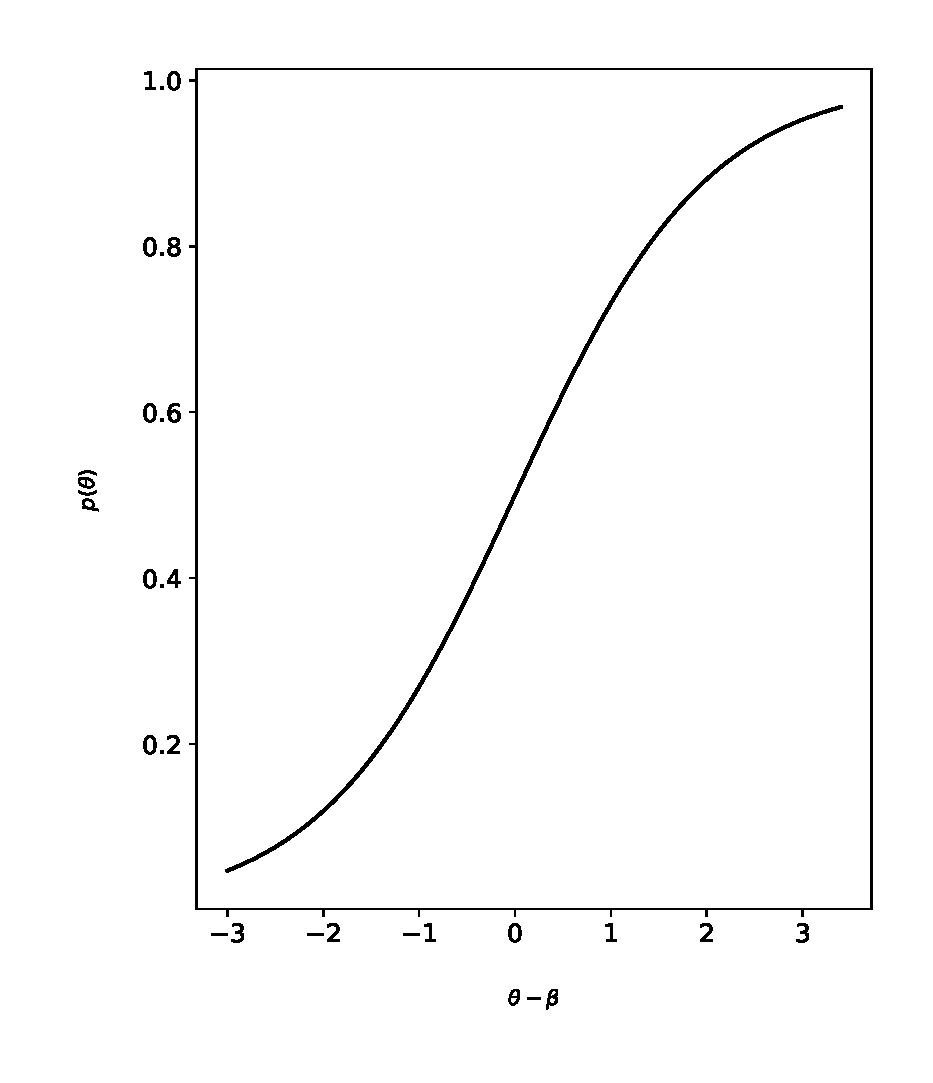
\includegraphics[width=.5\textwidth]{fig/irt.eps} 
   \caption{A probability curve in Item Response Theory.}
  \end{figure}
}



\frame{ \frametitle{Item Response Theory MLE}
  \begin{figure}[p!]
   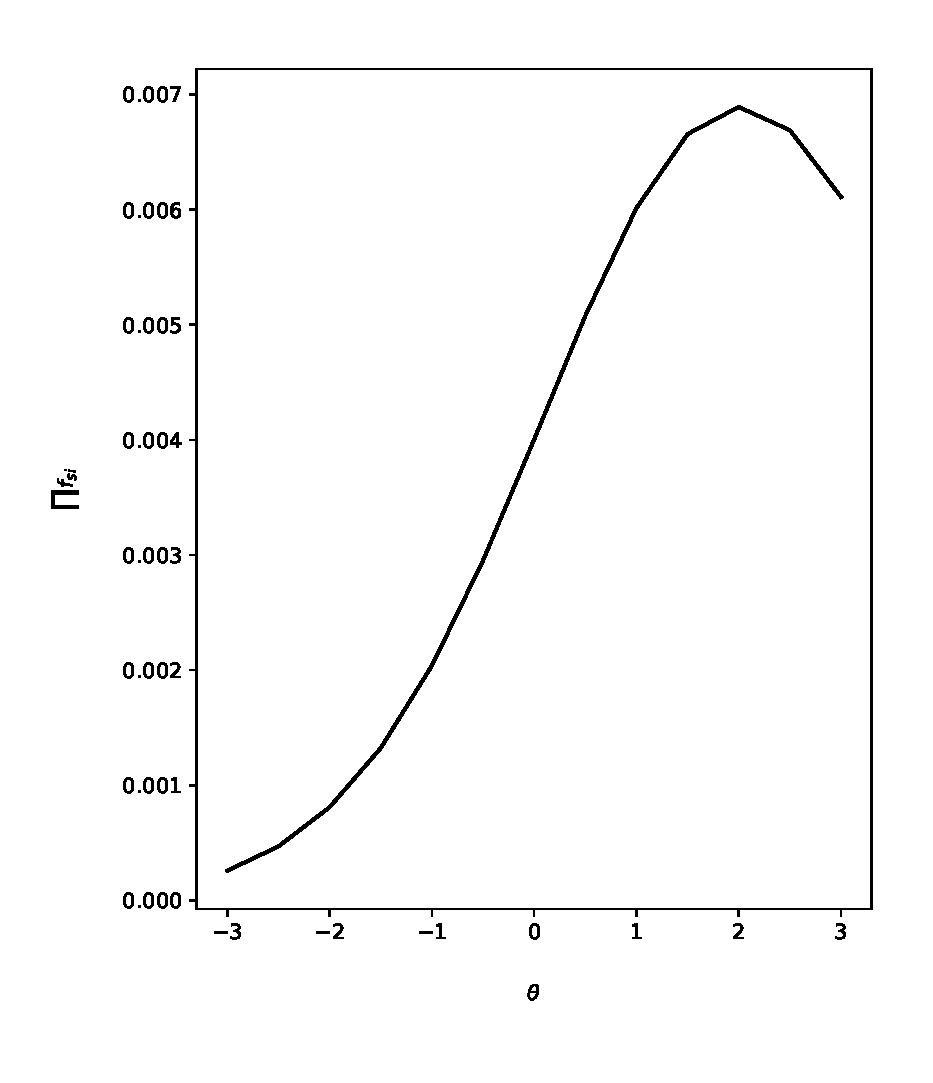
\includegraphics[width=.5\textwidth]{fig/mle.eps} 
   \caption{A maximum likelihood estimation with Item Response Theory.}
  \end{figure}
}



\frame{ \frametitle{Grades}
  \small
  \centering
  \begin{tabular}{||l|c|l||}
  \hline\hline
  Letter  & $\theta$  & Explanation \\\hline
  F  & -3.0   & unsatisfactory \\\hline
  D- & -2.5   &                \\
  D  & -2.0   & minimal        \\
  D+ & -1.5   &                \\\hline
  C- & -1.0   &                \\
  C  & -0.5   & acceptable     \\
  C+ & 0.0    &                \\\hline
  B- & 0.5    &                \\
  B  & 1.0    & good           \\
  B+ & 1.5    &                \\\hline
  A- & 2.0    &                \\
  A  & 2.5    & distinguished  \\
  A+ & 3.0    &                \\\hline\hline
  \end{tabular}
  \normalsize
}



\frame{ \frametitle{The Database}
  \begin{itemize}

    \item The database contains content items and assessments.

    \item Content items may be informative items or questions.  Both have an
    associated Bloom level, difficulty, and concept.  Questions have item
    discriminations, probabilities of guessing, and solutions.  All content
    items also have dependencies.

    \item Assessments are collections of item sets, which may be represented
    as trees.

  \end{itemize} 
}



\subsection{Literature}



\subsection{Previous Work}



\frame{ \frametitle{Difficulty and Bloom Level}
  \begin{itemize}

    \item It is widely thought that Bloom level and difficulty are strictly
    equal \cite{newman1988effect,oliver2004course,lord2007moving,
    johnson2006bloom,fuller2007developing} , but previous work
    \cite{castleberry2016effect} has argued the contrary, producing empirical
    evidence for the hypothesis that Bloom level and difficulty are separate
    entities.

    \item It is sufficient to find pairs of problems to serve as counterexamples:
    one at a higher Bloom level and lower difficulty than another, which has a 
    lower Bloom level and higher difficulty. 

  \end{itemize}
}



\section{Models and Data Structures}



\subsection{Representing Trait Ability}



\frame{ \frametitle{There are Multiple Abilities}
  \begin{itemize}

    \item A student may have differing levels of ability for different
    concepts.  A student may be good at recursion, but not at working with
    pointers.

    \item For that reason, trait ability should be separated per-concept.
    However, a student may have different levels of ability per Bloom level.

    \item For example, a student may have exceptional comprehension of
    recursion.  The student can follow a recursive procedure.  However, the
    same student may have low application ability; they cannot yet apply
    the rules of recursion to complete a fill-in-the-blank code.
    
  \end{itemize} 
}



\frame{ \frametitle{The Trait Ability Matrix}

  \begin{itemize}
    \item Since trait ability is per-student and per-Bloom level, the
    most representative data structure is a matrix:
  \end{itemize} 

  \[
  \Theta_s =\left[
           \begin{array}{lllll}
                \theta_{s11} & \ldots       & \ldots       & \ldots & \theta_{sn1}  \\
                \vdots       & \ddots       &              &        &               \\
                \vdots       &              & \theta_{sjk} &        &               \\
                \vdots       &              &              & \ddots &               \\
                \theta_{s1m} &              &              &        & \theta_{snm}  \\
           \end{array}
         \right]
  \]
}



\frame{ \frametitle{An Example Trait Ability Matrix}
  \begin{itemize}
   \item A likely matrix may look like the following, which has a
   diagonal gradient.  If the course follows a progression across Bloom
   levels and concepts, the student's ability per-concept and per-Bloom
   level should rise accordingly over time.
  \end{itemize}
  \[
  \Theta_1 =\left[
           \begin{array}{llllll}
               3 & 2.5 & 1   & 0   & -1     & -2   \\
               2 & 1.5 & 0   & -.5 & -1.5   & -2.5 \\
               1 &  .5 & 0   & -1  & -2     & -3   \\
               1 & 0   & -.5 & -1  & -2.5   & -3   \\
           \end{array}
         \right]
  \]
}



\subsection{Representing Dependencies}


\frame{ \frametitle{Question Dependencies}

  \begin{itemize} 
    \item  Some questions have dependencies.  Consider the following; one must
    know about integer division and the modulo operations before being able to
    combine them to solve problem (3).
  \end{itemize} 

  \begin{enumerate}
   \item \emph{What is (5 \% 2)?}
   \item \emph{What is (5 / 2)?}
   \item \emph{What is (5 \% (5 / 2))?}
  \end{enumerate}

  \begin{itemize} 
    \item  It is reasonable to assume that the student's ability to handle a
    a dependency (or a dependee) influences the ability to handle the question
    which depends on the dependencies (the depender).
  \end{itemize} 

}



\frame{ \frametitle{Identifying Potential Dependencies}

  \begin{itemize}
    \item If dependencies of the form $c \rightarrow a$ and $c \rightarrow b$
    exist (that is, $c$ depends on $a$ and $b$), they may be indicated by a
    high simple matching coefficient:
  \end{itemize} 

  \[
   \frac{n_{00} + n_{11}}{n_{00} + n_{01} + n_{10} + n_{11}}
  \]

  where the values for these various $n$ are:
  
 \begin{center}
 \begin{tabular}{|l|l|l|l|}
 \hline
        &  $y=0$         &  $y=1$         &  total     \\ \hline
   $x=0$ & $n_{00}$      & $n_{01}$      & $n_{0 \bullet }$  \\ \hline
   $x=1$ & $n_{10}$      & $n_{11}$      & $n_{1 \bullet }$  \\ \hline
   total & $n_{\bullet 0}$ & $n_{\bullet 1}$ & $n$                \\ \hline
 \end{tabular}
 \end{center}


}



\frame{ \frametitle{Identifying Dependencies}

  \begin{itemize} 

    \item Alternatively, the phi coefficient, or mean square contingency
    coefficient, can be used to identify the degree of association between two
    questions.  It is defined as:

    \[
     \phi = \frac{n_{11}n_{00} - n_{01}n_{10}}
     { 
       \sqrt{ n_{\bullet 0} n_{\bullet 1} n_{0 \bullet} n_{1 \bullet} } 
     }
    \]

    \item This is the binary analogue to the Pearson correlation coefficient;
    but its range is only $[-1, 1]$ if there is a fifty-fifty split.  

  \end{itemize} 


}


\frame{ \frametitle{Assessments are Forests}
  \begin{figure}[!p]
    \centering\includegraphics[width=.6\textwidth]{fig/forest.eps}
  \caption{A forest obtained from an item set, where each tree is a subset
  of the item set which has dependency relationships}
  \end{figure}
}



\frame{ \frametitle{Some ``Dependencies'' are Not Dependencies}
  \begin{figure}[!p]
    \centering\includegraphics[width=.6\textwidth]{fig/severance.eps}
  \caption{The severance of dependency relationships based upon low $\alpha$
  values}
  \end{figure}
}



\frame{ \frametitle{The Base Graph}
  \begin{figure}[!p]
    \centering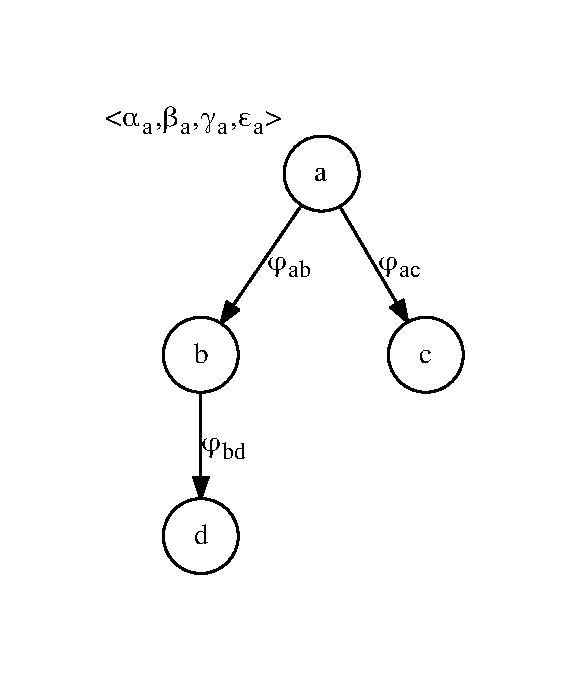
\includegraphics[width=.4\textwidth]{fig/base-graph.eps}
  \caption{The base item set graph, which includes item-specific paramters}
  \end{figure}
}



\frame{ \frametitle{The Student Graph}
  \begin{figure}[!p]
      \centering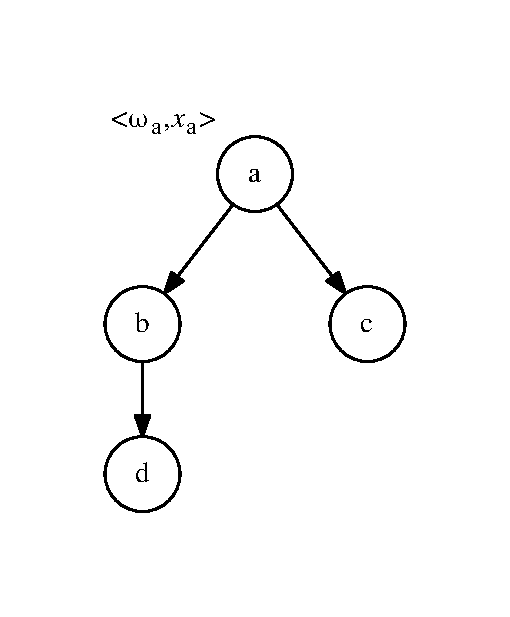
\includegraphics[width=.3\textwidth]{fig/student-graph.eps}
  \caption{The student-specific item set graph, which includes the list of
  student responses and timestamps for each response}
  \end{figure}
}



\subsection{Logistic Regression}


\frame{ \frametitle{Linear Regression}

   \begin{itemize}
     \item We might consider the use of linear regression to determine
     whether or not a student will answer a question correctly ($Y$) 
     given responses for $X_1$, $X_2$, etc.

     \item Consider the linear equation in which a binary dependent variable
     $Y$ depends on some response $X$:
   \end{itemize} 

  \[
           Y = a + bX + \epsilon
  \]

}



\frame{ \frametitle{We Shouldn't Use Linear Regression}

  \begin{itemize}

    \item Unfortunately, our particular scenario violates a few of the
    assumptions required for linear regression.  

    \item There is no linear relationship since our dependent variable is 
    categorical (0 or 1).

    \item Every linear combination of components should have a univariate 
    normal distribution, but every component only assumes one of two possible
    values.

    \item Linear regression requires homoscedasticity.  The error terms along
    the regression should be equal, but in the above situation, the variance of
    the error is dependent on the probability.   In particular
    $\mathrm{var}(\epsilon) = p(1-p)$.

  \end{itemize} 

}




\frame{ \frametitle{We Should Use Logistic Regression}

  

}




\frame{ \frametitle{The Assumptions of Logistic Regression}

  \begin{itemize} 

   \item The dependent variable is binary,
   
   \item P(Y=1) is the probability that the event $Y$ occurs, 
   
   \item The model is fitted correctly, which means that there are no extraneous
   variables used in the regression, but that all variables are meaningful,

   \item That error terms should be independent; each observation should be
   independent, and little to no multicollinearity should exist.  

   \item Indepedent variables should be linearly related to the log odds of
   the event.

  \end{itemize} 

}



\frame{ \frametitle{Possible Violations}

  \begin{itemize} 

   \item The user can extraneous variables by examining $\alpha$, and specifies
   the graph from the outset, so there \emph{shouldn't} be extraneous
   variables.

   \item Some multicollinearity will probably exist for most dependency sets 
   due to the nature of the dependee-depender relationships.

   \item An extraction technique like PCA or factor analysis could be done to
   avoid multicollinearity, but then the graphs would not be as legible.  Plus,
   we would need to do PCA/FA every time the question is answered, which can be
   expensive.

 \end{itemize} 

}


\frame{ \frametitle{Logistic Regression: The Math}

  Logistic regression is a regression of what are known as log odds. The odds
  are defined as:

  \[
    \mathrm{odds} = \frac{p}{1-p}
  \]

  And the log odds, or logit, is defined as:

  \[
    \logit(y) = \ln(\mathrm{odds}) = \ln\Big(\frac{p}{1-p}\Big) = a + bX
  \]

}



\frame{ \frametitle{The Logistic Curve and Item Response Theory}

  Correspondingly, odds may be defined as follows:

  \[
    \frac{p}{1-p} = e^{a + bx}
  \]

  Solving this equation for $p$ yields

  \[
    p = \frac{e^{a + bx}}{1 + e^{a + bx}}
  \]

  which can be reduced to 

  \[
    p = \frac{1}{1 + e^{-(a + bx)}}
  \]

  which is called the logistic curve, which is one in the family of sigmoid
  curves.  It is identical to the type of curve used in Item Response Theory:

  \[
    a + bx = \alpha(\beta - 1)\theta
  \]

}


\frame{ \frametitle{The Inclusion of Dependency Information}

  To account for item dependencies, a modified form of logistic regression may be
  sought.  It is desirable to keep in account the item discrimination as well as
  the trait ability of the student.  Here, $X_i$ is the correctness of the
  $i^{th}$ dependee response, and $Y$ is the log odds that the depender question
  is answered correctly:
  % FIXME

  \[
    Y = b_1X_1 + b_2X_2 + \ldots + b_{n-1}X_{n-1} + b_n\alpha_i(\theta_s-\beta_i)
  \]

}



\frame{ \frametitle{A Neural Network}
  \begin{figure}[!p]
    \centering\includegraphics[width=.5\textwidth]{fig/neural.eps}
  \caption{A perceptron; a single-layer neural network, where the inputs a, b, and c
  are multiplied by weights, summed, and applied to a sigmoid squash function}
  \end{figure}
}



\frame{ \frametitle{The Dependency Graph with Weights}
  \begin{figure}[!p]
    \centering\includegraphics[width=.5\textwidth]{fig/deps.eps}
  \caption{A view of the dependency graph and weights used in the logistic regression,
  including the item parameters}
  \end{figure}
}



\subsection{Memory Models}



\frame{ \frametitle{Law of Forgetting}

  \begin{itemize} 

    \item Ebbinghaus is credited with a theory of memory and forgetting which
    has withstood empirical study for over a century \cite{ebbinghaus}, known
    as the power law of forgetting, according to which the strength of a memory
    after a time $t$ falls off exponentially: 

  \end{itemize} 

  \[
   S(t) = ae^{-bt}
  \]

  \begin{itemize} 
    \item In this model, $a$ is the initial strength of the memory, and
    $b^{-1}$ is a decay rate.  If $a=1$, the function may be interpreted as a
    probability function:
  \end{itemize} 

  \[
   p_{recall}(t) = e^{-bt}
  \]

}



\frame{ \frametitle{The Curve of Forgetting}
  \begin{figure}[p!]
   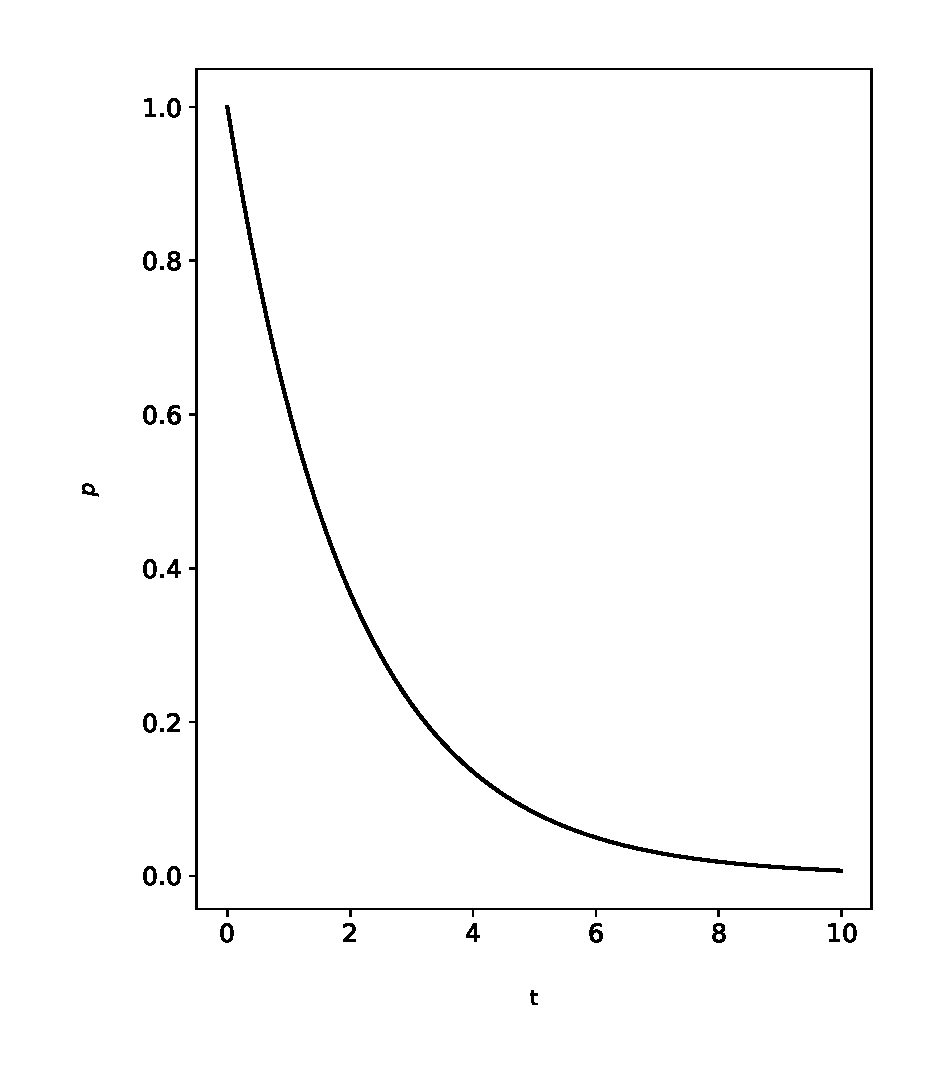
\includegraphics[width=.4\textwidth]{fig/forgetting.eps} 
   \caption{The Ebbinghaus curve of forgetting, which features an exponential
   dropoff of memory strength over time}
  \end{figure}
}



\frame{ \frametitle{The Modified Curve of Forgetting}
  \begin{figure}[p!]
   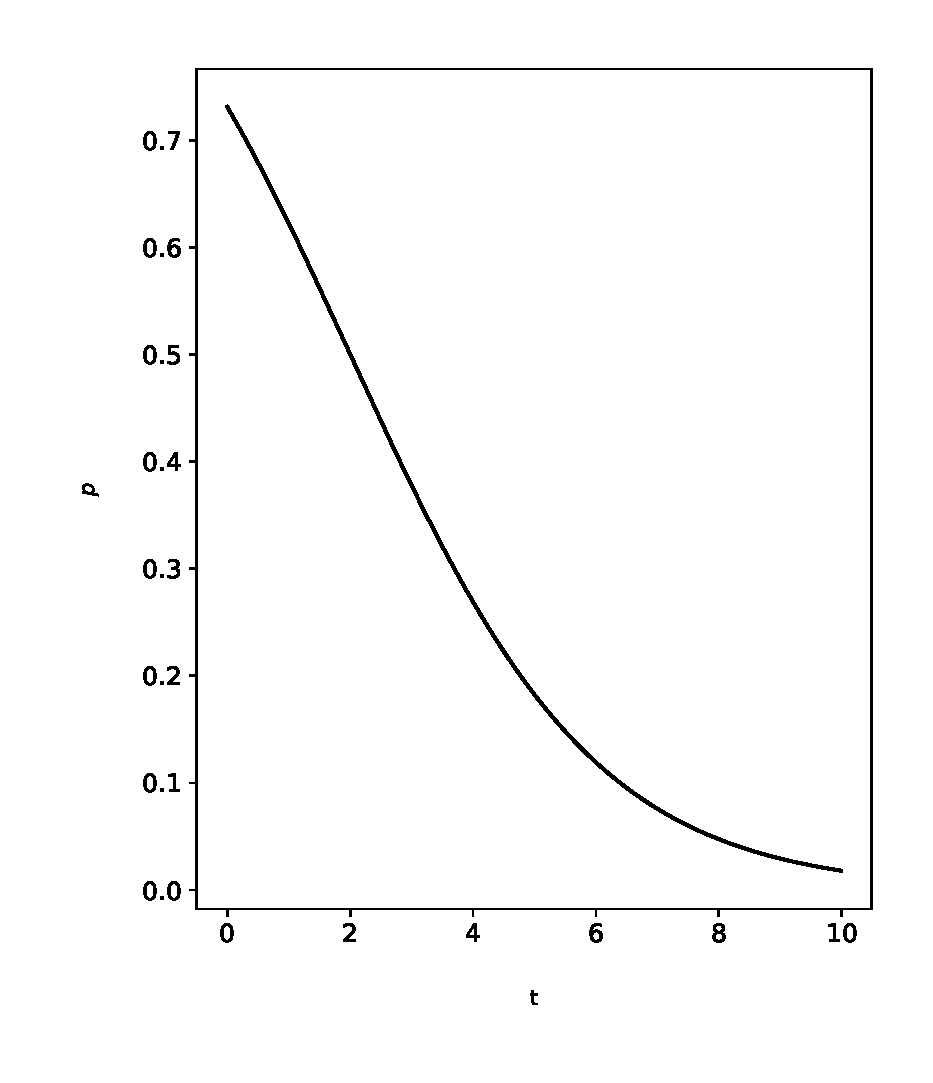
\includegraphics[width=.4\textwidth]{fig/modified.eps} 
   \caption{The modified curve of forgetting, which resembles the reverse
   sigmoid function}
  \end{figure}
}



\frame{ \frametitle{ACT-R}

  \begin{itemize} 

    \item John Anderson is credited with having developed Adaptive Control of
    Thought-Rational (ACT-R), a process-based model which simulates the solving
    of problems.  In ACT-R, there are goals, akin to problem statements; and
    rules, or processes used to solve problems; and finally facts, or knowledge
    utilized in the course of applying rules. 

    \item In addition to this, however, Anderson added models for memory and
    forgetting to support realistic recall probabilities and latencies, some
    of which inspire the present work.

  \end{itemize} 

}


\frame{ \frametitle{Anderson's Activation via Related Concepts}

  \begin{itemize} 
    \item According to Anderson's model, a chunk of memory $i$ is re-activated
    (or additionally activated) to the extent that other chunks of information
    (related concepts, words, ideas, etc.) which have some association to $i$
    are attended to.  This notion is captured in the following equation
    \cite{anderson2000implications}:
  \end{itemize} 

  \[
    a_i = b_i + \displaystyle\sum_{i=j}^n w_j s_{ji}
  \]

}

\frame{ \frametitle{The Effect of Practice}

  \begin{itemize} 
    \item Practice has the effect of causing the base strength of the memory to
    increase, and delays cause the strength of the memory to drop off
    \cite{anderson2000implications}:  
  \end{itemize} 

  \[
    b_i = \mathrm{ln} \Bigg( \displaystyle\sum_{j=1}^n t_j^{-d} \Bigg)
  \]

  \begin{itemize} 
    \item Here, $t_j$ is the time since the jth practice of an item, and $d$ is
    a decay rate. 
  \end{itemize} 

}



\frame{ \frametitle{Forgetting with Re-Activation}
  \begin{figure}[p!]
   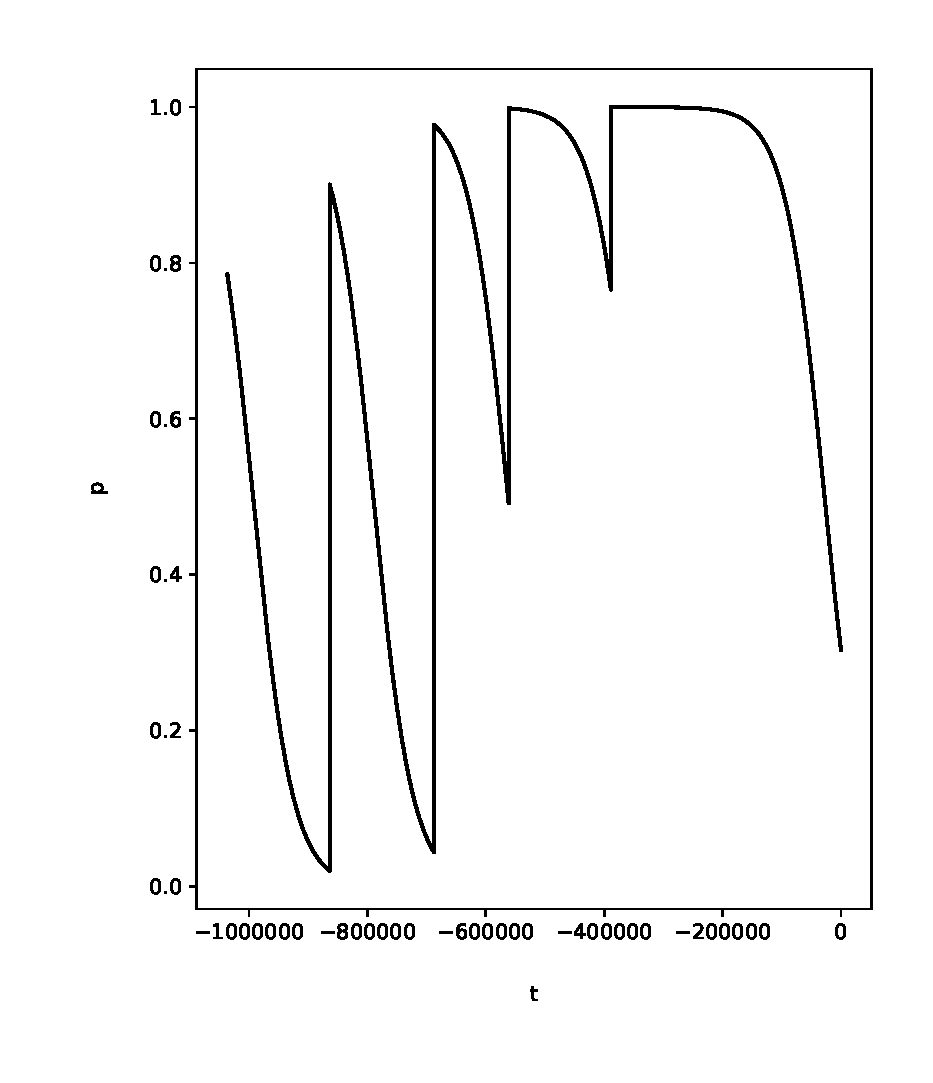
\includegraphics[width=.4\textwidth]{fig/memory.eps} 
   \caption{Forgetting with re-activation; each spike in the graph is an
   additional trial where the student is exposed to the item again}
  \end{figure}
}



\frame{ \frametitle{Learning Curve}
  \begin{figure}[p!]
   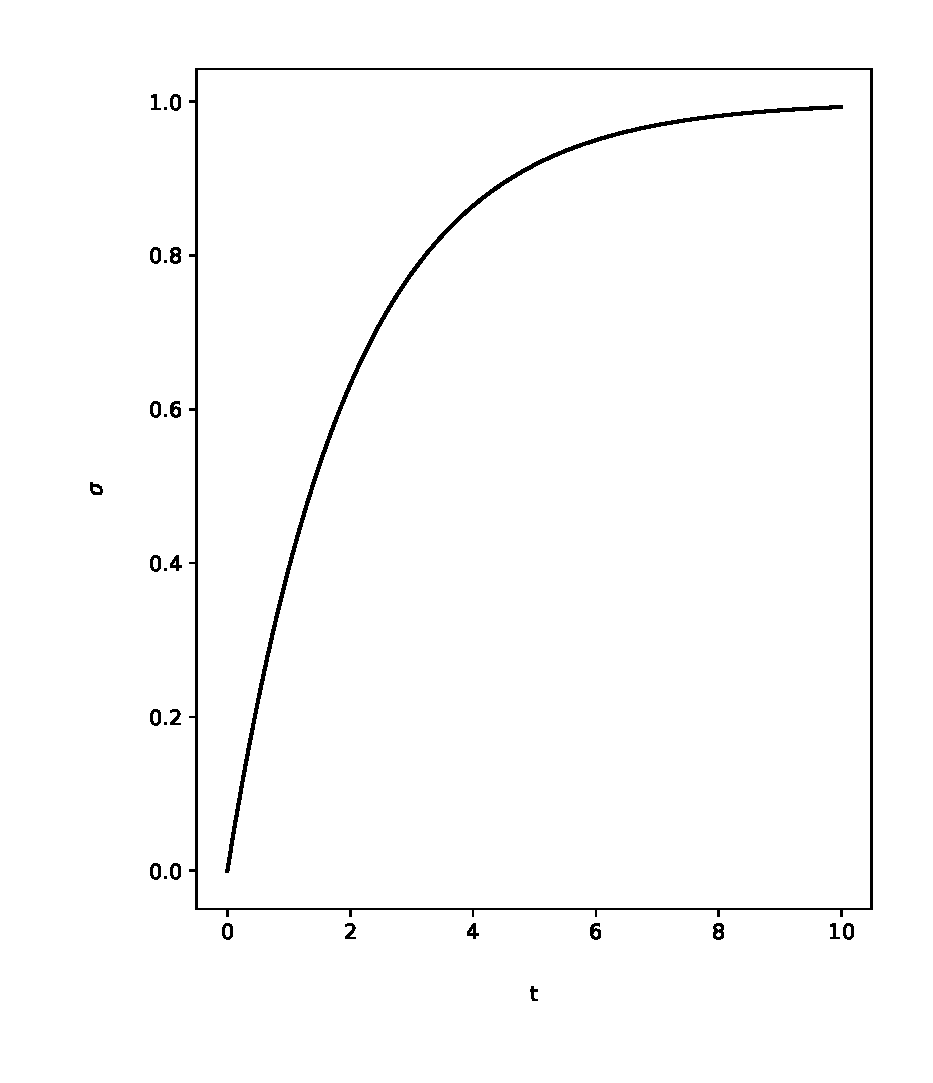
\includegraphics[width=.4\textwidth]{fig/spacing.eps} 
   \caption{The learning curve, which indicates the extent of memory
   lifespan increase given a time between trials}
  \end{figure}
}



\frame{ \frametitle{A Modification to the Memory Models}
  
  \begin{itemize} 
    \item A slight modification to this theory accounts for short-term memory
    and short-term memorization, which allows for a small time window for the
    student to enjoy a high probability of recollection before dropping off
    sharply, as in the original curve:
  \end{itemize} 

  \[
    p_{recall}(t) = \frac{1}{1 + e^{{m(t-\lambda)}}}
  \]

  \begin{itemize} 
    \item In this equation, $\lambda$ is the lifespan of the memory; or, the
    amount of time that passes until there remains only a .5 probability that
    the student recalls the information.  The value $m$ is a parameter which
    controls the rate of dropoff, much like the decay rate in Ebbinghaus'
    model.  An example curve for this equation is given below.
  \end{itemize} 

}



\frame{ \frametitle{Re-Activation}

  \begin{itemize} 
    \item To account for re-activation, a simple model for the extension of
    half-life may be used: 
  \end{itemize} 

  \[
   \lambda_n = \rho_s \lambda_{n-1}
  \]

  \begin{itemize} 
    \item Here, $n$ refers to exposure or trial number $n$.  In the intelligent
    tutoring system, this is the nth time that the student has seen the
    problem.  $\lambda_{n-1}$ is the former lifespan of the memory.  $\rho_s$
    is a learning rate, which is a parameter particular to the student; its
    domain is (1, $\infty$].  The intuition captured by this formula is that
    with an increased number of trials, the lifespan of the memory increases.
  \end{itemize} 

}



\frame{ \frametitle{Forgettability}
  \begin{itemize} 
    \item In addition, there is a difference in problems in the ease with which
    they are learned.  An addendum to this can be used to account for
    individual differences in problems: 
  \end{itemize} 

  \[
   \lambda_n = \mu_i \rho_s \lambda_{n-1}
  \]

  \begin{itemize} 
    \item Here, $\mu_i$ represents the memorability of the problem, or the ease
    with which the problem solution can be committed to memory. 
  \end{itemize} 
}



\frame{ \frametitle{The Spacing Effect}
  \begin{itemize} 
    \item The spacing effect is the effect that the amount of time in between
    trials has on the memorization of a chunk of memory.  In the above model,
    memorization is interpreted as an increase in the lifespan of a memory.  If
    only a short amount of time passes between the last trial, the effect will
    not be as great as if a longer time has passed.  
    
    \item One consequence of this is that, according to the spacing effect
    hypothesis, cramming is ineffective (where cramming is namely repeating
    trials in short bursts).

    \item The spacing effect can be accommodated in the memory model used by the
    intelligent tutoring system.  We define a function for the dropoff:
  \end{itemize} 

  \[
    \sigma_t = (1 - e^{-at})
   \]

}



\frame{ \frametitle{The Lifespans of Memories}
  \begin{itemize} 
    \item This function indicates the extent to which the spacing from the time
    the item was last seen influences the increase in the lifespan of the
    memory: 
  \end{itemize} 

  \[
   \lambda_n = (1 + \sigma_t \mu_i \rho_s) \lambda_{n-1}
  \]

  \begin{itemize} 
    \item The utility of this model is in assessing the probability with which a
    student answers a question; not only based on trait ability and dependency
    relationships, but also on the inherent tendency to forget information with
    the passage of time.
  \end{itemize} 
}


\frame{ \frametitle{Remember or Re-Solve}
  \begin{itemize} 
  \item It will be assumed that, if a student has been exposed to a item before, then
  the probability of being able to answer the item correctly may assume one of
  two values.  

  \item The first is based upon recollection; it is the probability of
  recalling the facts, processes, and so forth required to produce the solution
  for an item.  

  \item The second is based upon derivation of the solution from known
  facts, processes, and so forth in the dependencies, as if the student were
  answering the question for the first time.  
  \end{itemize} 
}


\frame{ \frametitle{Remember or Re-Solve}

  \begin{itemize} 
    \item That is, if a student does not recall the process for solving a
    problem, the probability defaults to the probability based upon item
    parameters, trait ability and dependency relationships:
  \end{itemize} 

  \[
  p =\left\{
           \begin{array}{ll}
                 p_{recall}(t) & \mathrm{if}\  p_{recall} > p({\theta_s, x_1, \ldots}) \\
                 p({\theta_s, x_1, \ldots}) & \mathrm{otherwise}
           \end{array}
         \right.
  \]

}



\section{Algorithms for Scheduling}



\subsection{Selecting From the Trait Ability Matrix}


\frame{ \frametitle{Initialization}
  \begin{itemize} 
    \item First, at the very beginning of the program, the trait ability matrix
    for the student is initialized:
  \end{itemize} 

  \begin{equations}
    \Theta \leftarrow -3
  \end{equations}
  
}





\frame{ \frametitle{How to Select Categories}
  \begin{itemize}

    \item Categories with $\theta_{sjk} = 0$ are areas where the student has a
    roughly .5 probability of answering a question of difficulty $\beta=0$
    correctly.

    \item Knowing what the trait ability matrix looks like, what
    categories should be selected?

  \end{itemize} 
}




\frame{ \frametitle{Too Easy: Don't Bother}
  \begin{itemize} 

    \item The higher $\theta_{sjk}$ values should be left alone, particularly
    those nearing 3, since this demonstrates exceptional mastery of that (Bloom
    $\times$ concept) category.  In particular, if $\theta_{sjk} = 3$, there is
    no reason to ask questions from that category, since trait ability is
    capped at 3.

    \item As will be discussed later, there may be precedent to ask such a
    question if asking it will lead to an increase in the probability of
    answering other questions.

  \end{itemize} 
}



\frame{ \frametitle{Too Hard: The Potential for Cruelty}
  \begin{itemize} 

    \item It would be unfair (perhaps even cruel), to ask questions for which
    $\theta_{sjk}-\beta>1$; that is, those questions for which the student has
    a less than half chance of answering correctly.  Asking such questions
    consistently could have psychological ramifications.

    \item In the course of ordinary non-formative instruction, such questions
    may be asked, but in this case the schedule may be personalized and the
    probabilities of success are known.

  \end{itemize} 
}
 


\frame{ \frametitle{Just Right: Where p~.5}
  \begin{itemize}  

    \item The difficulty matrix for the student may be

    \[
      B_s = \Theta_s - \delta
    \]

    where $\delta$ is some (small) number.  The smaller the number, the
    harder the questions relative to the student's ability; but also the
    fewer that the student must answer to raise their trait ability estimate.

    \item Ultimately, selecting the neighborhood of difficulties to include
    questions from is a personal decision.  If the question bank is
    well-populated, it shouldn't affect scoring. 

  \end{itemize} 
}



\subsection{Auto-Grading}



\frame{ \frametitle{Short Answer Distance Metrics}
  \begin{itemize}
    \item Lehvenstein distance \ldots
  \end{itemize} 
}


\frame{ \frametitle{A Simple Code Autograder}
 \begin{align*}
  \langle expr \rangle_1 & \rightarrow  x_1 \\
  \langle expr \rangle_2 & \rightarrow  x_2 \\
                         & \vdots       \\
  \langle expr \rangle_i & \rightarrow  x_i \\
                         & \vdots       \\
  \langle expr \rangle_n & \rightarrow  x_n 
 \end{align*}
}



\section{Experiments and Conclusion}

\subsection{Experiment 1}

\frame{ \frametitle{\ldots}
  \ldots
}


\subsection{Experiment 2}

\frame{ \frametitle{\ldots}
  \ldots
}



\end{document}
